\cleardoublepage
\chapter{Safely learning with kernels}
\markboth{Learning with kernels}{Learning with kernels}

In this chapter, we will introduce the problem of learning from data and elucidate what approach will be taken to tackle it. Next, novel uncertainty quantification results will be presented concerning the point-evaluations of an  unknown ground-truth. Finally, some examples are given to illustrate the general use of the theory.

\section{The problem of learning}

At its core, learning refers to the process of \textit{gathering information} and using it to \textit{improve one's knowledge} about the subject or phenomenon under study. The standing assumption here is then clearly that a link is in place, tying information and phenomenon together, even if such link is partially corrupted.

Information comes in many science fields in the form of data, samples, sometimes referred to as examples. In modern machine learning, people study a number of rather abstract subjects ranging from the traits that distinguish images of muffins and chihuahuas, to the link between passengers' features and their survival likelihood in case of a ship sinking event.  The mathematical formalism often used to study the link between examples and these phenomena is statistics. This choice is convenient because it can describe the possible non-determinism of outcomes through the concepts of distributions and samples; and because it provides us with plenty of tools to carry out learning, i.e., improve our knowledge about the phenomenon through the samples at hand. In this chapter, we will however adopt a different standpoint to study and tackle the problem of learning, which is, as we will later argue, more aligned with the ways control engineers are taught to see physical systems. This standpoint is the one offered by approximation theory.

\mycomment{Statistical learning and approximation theory are not in opposition. Indeed, we can define the function of interest as the conditional \cite{temlyakov2008approximation}, perhaps talk about Belkin's work linking the two and advocating for using the approximation lenses.}

\section{The formalism of kernels}
\label{sec.formalism_of_kernels}

\begin{definition}
	\textbf{(Kernel)} Given an arbitrary non-empty set $\mathcal{X}$, a kernel $k$ is any symmetric function of the form
	\begin{equation}
		k: \mathcal{X} \times \mathcal{X} \rightarrow \mathbb{R}
	\end{equation}
\end{definition}

\begin{figure}[t]
	\centering
	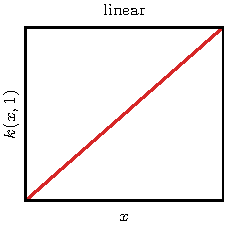
\includegraphics[scale=0.4]{../images/chap2_kernel_li.pdf} \hspace{3pt}
	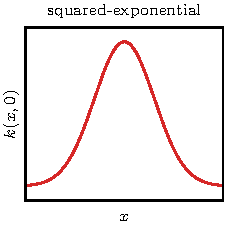
\includegraphics[scale=0.4]{../images/chap2_kernel_se.pdf} \hspace{3pt}
	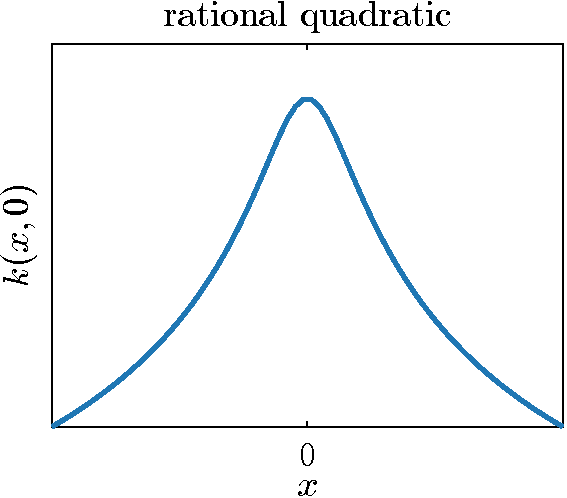
\includegraphics[scale=0.4]{../images/chap2_kernel_rq.pdf} \\[3pt]
    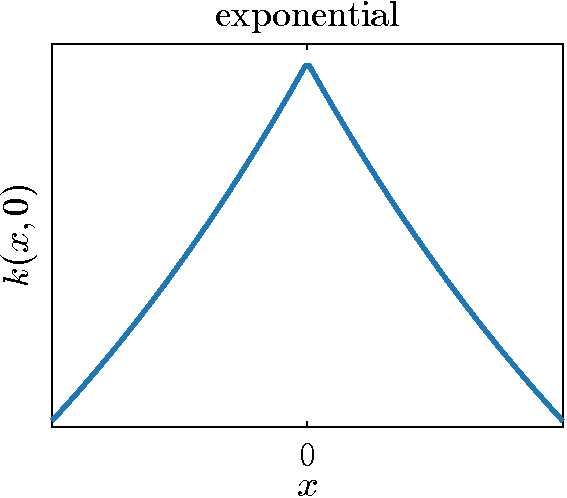
\includegraphics[scale=0.4]{../images/chap2_kernel_ex.pdf} \hspace{3pt}
    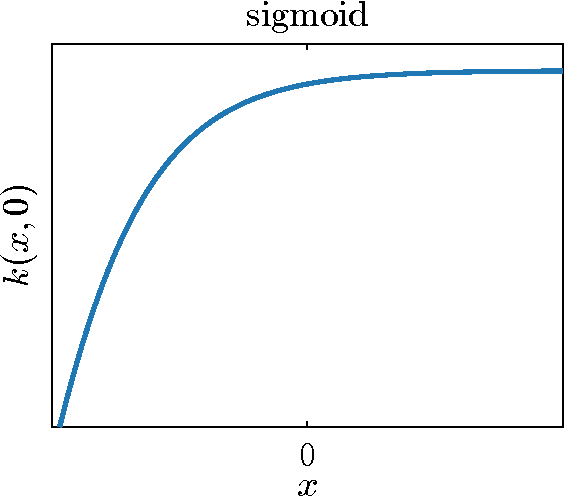
\includegraphics[scale=0.4]{../images/chap2_kernel_sg.pdf} \hspace{3pt}
    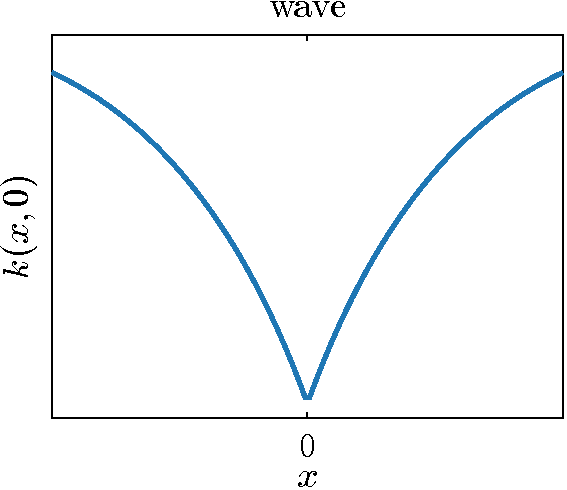
\includegraphics[scale=0.4]{../images/chap2_kernel_wv.pdf} 
	\caption{Examples of positive-definite kernels.}
	\label{fig.pd_kernels}
\end{figure}

\begin{definition}
	\textbf{(Kernel matrix)} Let $X = \{x_1,\dots,x_n\} \subset \mathcal{X}$ be a finite set of points. The $n \times n$ matrix $K_{XX}$ with entries $[K_{XX}]_{ij} = k(x_i,x_j)$ is called the kernel matrix of $k$ associated with $X$.
\end{definition}


\begin{definition}
	\label{def.pd_kernel}
	\textbf{(Positive-definite kernel)} A kernel function $k$ is said to be positive-definite if for any finite subset of points $X \subset \mathcal{X}$, the kernel matrix satisfies $K_{XX} \succeq 0$. If, in particular, $K_{XX} \succ 0$, then the kernel is strictly positive-definite.
\end{definition}

Aside from the last definition, we underline that there exist broader classes of kernel functions such as the \textit{conditionally positive-definite} one \cite[§2.4]{scholkopf2002learning}\cite[§8]{wendland2004scattered}. In this chapter however, our attention will be focused on the positive-definite (PD) set, from which some examples are shown in Figure~\ref{fig.pd_kernels}. A more complete list of PD kernels and their mathematical properties can be found in Appendix~A.

Recall that our original goal was to learn functions $f: \mathcal{X} \rightarrow \mathbb{R}$. With a kernel at hand, one can define functions with the same domain and co-domain simply by \textit{partially evaluating} $k$, in other words, fixing one of its arguments: for some $z \in \mathcal{X}$, we can define $k(z,\cdot): \mathcal{X} \rightarrow \mathbb{R}, x \mapsto k(z,x)$. Indeed, this was the approach taken to draw the plots in Figure~\ref{fig.pd_kernels}. Approximating the unknown ground-truth with a single partially evaluated kernel however appears to be overly restrictive. The next logical step is to consider a larger hypothesis space where our approximation is given by a linear combination of such kernel functions. It turns out that every PD kernel already has a similar space associated with it, which is complete and endowed with enough structure to allow us to develop our uncertainty quantification theory. The following concepts are presented next to set up the stage for defining this special hypothesis space, the \textit{reproducing kernel Hilbert space}.

\mycomment{Talk about feature maps, liftings and their importance.}

\begin{proposition}
	\label{thm.pd_kernels_feature_maps}
	\textbf{(PD kernels have feature maps)} 
	Let $k:\mathcal{X} \times \mathcal{X} \rightarrow \mathbb{R} $ be a positive-definite kernel. Then there exists a Hilbert space $\mathbb{H}$ endowed with an inner product $\langle \cdot,\cdot \rangle_\mathbb{H}$ and a mapping $\Phi :  \mathcal{X} \rightarrow \mathbb{H}$ such that 
	\begin{equation}
		k(x,x') = \langle \Phi(x),\Phi(x') \rangle_\mathbb{H}
	\end{equation}
	holds for any $x,x' \in \mathcal{X}$.
\end{proposition}

\begin{my_proof}
	\cite[Theorem~4.16]{steinwart2008svm_book}, modulo the nomenclature difference.
\end{my_proof}

The mappings $\Phi$ above as well as the $\mathbb{H}$ spaces are in general not unique \citep[§4]{steinwart2008svm_book}, but there is one such space that enjoys an extra property that rules out some unexpected behavior from its members. This concept is introduced next.

\begin{definition}
	\label{def.rkhs}
	\textbf{(Reproducing kernel Hilbert space)} 
	Let $\mathcal{X} \neq \emptyset$ and $\mathbb{R}^\mathcal{X}$ the set of functions mapping $\mathcal{X}$ to $\mathbb{R}$. The subset $\mathcal{H} \subset \mathbb{R}^\mathcal{X}$ is called a reproducing kernel Hilbert space (RKHS) if it is a Hilbert space and if $\forall x \in \mathcal{X}$ the evaluation functionals
	\begin{equation}
		L_x: \mathcal{H} \rightarrow \mathbb{R}, \; L_x(f) \mapsto f(x), \ \forall f\in \mathcal{H}
	\end{equation}
	are bounded.
\end{definition}

In order to see how useful such a property is, consider a sequence $\{f_n\}_{n=1}^\infty$ within a certain Hilbert function space $\mathbb{H} \subset \mathbb{R}^\mathcal{X}$. Intuitively, one would expect that if $f_n \rightarrow f^\star$ in $\mathbb{H}$, then the values $f_n(x)$ attained by the sequence would converge to the values $f^\star(x)$. Yet, this is not always the case (see Example~\ref{ex.appendix_convergence} in Appendix~\ref{app.elements_analysis_algebra}). If, on the other hand, the evaluation functionals are bounded as in Definition~\ref{def.rkhs}, then the connection between convergence in the function space and the pointwise convergence of functions is guaranteed. Indeed, if $\{f_n\}_{n=1}^\infty$ and $f^\star$ are members of an RKHS $\mathcal{H}$, then $|f_n(x)-f^\star(x)| = | L_x(f_n) - L_x(f^\star)|  \leq \Vert L_x \Vert \rknorm{f_n - f^\star}$. $\Vert L_x \Vert $ is the operator norm of $L_x$, which is guaranteed by Definiton~\ref{def.rkhs} to be a finite number, and $\rknorm{f_n - f^\star} \rightarrow 0$. Therefore, function convergence in an RKHS implies pointwise convergence, matching our intuition.

\begin{proposition}
	\label{prop.unique_reprod_kernel}
	\textbf{(Every RKHS has a unique PD reproducing kernel)} 
	Let $\mathcal{H} \subset \mathbb{R}^\mathcal{X}$ be an RKHS. Then, the map $k: \mathcal{X} \times \mathcal{X} \rightarrow \mathbb{R}$, $k(x,x') := \langle L_x, L_{x'} \rangle_\mathcal{H}$ is a positive-definite kernel. Furthermore, $k$ is the unique map to satisfy the reproducing property, i.e., for any $x \in \mathcal{X}$, $k(x,\cdot) \in \rkhs$ and
	\begin{equation}
		\rkinner{f}{k(x,\cdot)} = L_x(f) = f(x), \ \forall f \in \rkhs
	\end{equation} 
\end{proposition}

\begin{my_proof}
	 \cite[Lemma~2]{berlinet2011reproducing} along with \citep[Theorem~4.20]{steinwart2008svm_book}.
\end{my_proof}

\begin{proposition}
	\label{prop.unique_rkhs}
	\textbf{(Every PD kernel has a unique RKHS)} 
	Let $k: \mathcal{X} \times \mathcal{X} \rightarrow \mathbb{R}$ be a PD kernel. If $k$ is the reproducing kernel of an RKHS $\rkhs_A$ and of another RKHS $\rkhs_B$, then $\rkhs_A = \rkhs_B$.
\end{proposition}

\begin{my_proof}
	\citep[Theorem~4.21]{steinwart2008svm_book}.
\end{my_proof}

Despite being part of their name, it is not clear from the definition above what the relationship between RKHSs and kernels is. To shed light on the matter, it helps to explicitly construct $\rkhs$ starting from a given $k$. Consider the so-called \textit{pre-Hilbert space}
\begin{empheq}[box={\mymathbox[colback=black!2,drop small lifted shadow, sharp corners]}]{align}
	\rkhs_0 :=& \; \text{span} \, \{ k(x,\cdot) \, | \, x \in \mathcal{X} \} \\
 	=&  \; \left\{ \sum_{i=1}^n c_i \, k(x_i,\cdot) \, | \, n \in \mathbb{N}, c_i \in \mathbb{R}, x_i \in \mathcal{X} \right\} \label{eq.pre_rkhs}
\end{empheq}
equipped with the real-valued map $\langle f,g\rangle_{\mathcal{H}_0} := \sum_{i=1}^n \sum_{j=1}^m a_i b_i k(x_i,x_j)$, which can be shown to be a valid inner-product, for members $f,g \in \mathcal{H}_0, f=\sum_{i=1}^n a_i \, k(x_i,\cdot), g=\sum_{j=1}^m b_j \, k(x_j,\cdot) $. This family $\mathcal{H}_0$ of functions is however not guaranteed to be complete, i.e., sequences $\{f_i\}_{i\in\mathbb{N}}$ of members might converge to functions outside $\mathcal{H}_0$. To transform it into a proper Hilbert space, one closes the space 
\begin{empheq}[box={\mymathbox[colback=black!2,drop small lifted shadow, sharp corners]}]{equation}
	\label{eq.rkhs_closure}
	\mathcal{H} := \text{clos} \, \mathcal{H}_0
\end{empheq}
%\begin{equation}
%	\mathcal{H} := \text{clos} \, \mathcal{H}_0
%\end{equation}
thus encompassing all limit points\footnote{
%
Closing $\mathcal{H}_0$ requires defining an inner-product on the superset $\rkhs$ that is consistent with the one present in the subset $\mathcal{H}_0$. Also, the closure of a set is always closed, which guarantees that sequences within $\mathcal{H}$ cannot converge to functions outside of it.
%
}. Finally, the function space $\mathcal{H}$ defined in \eqref{eq.rkhs_closure} can then be shown to be a valid RKHS\footnote{
%
For a proof of this statement, the reader is referred to \cite[§3]{berlinet2011reproducing}, or to \cite[§4]{sejdinovic2012rkhs} for a more step-by-step pedagogical exposition.
%
} according to Definition~\ref{def.rkhs}, in fact, the only RKHS associated with $k$. We therefore understand that the members of $\rkhs$ are weighted sums of partially evaluated kernels as per \eqref{eq.pre_rkhs} along with their limit points. 
%and requires showing that the elements included through the closure are indeed functions with well-defined point evaluations \cite[§4]{aronszajn1950theory}\cite[§10.2]{wendland2004scattered}, a step that is overlooked in simplified presentations.

\begin{definition}
	\textbf{(Universal kernel)}
	Let $k$ be a continuous PD kernel and the set $\mathcal{X}$ be a compact metric space. Then $k$ is called universal if its RKHS $\rkhs \subset \mathbb{R}^\mathcal{X}$ is dense in the space of real-valued continuous functions $C(\mathcal{X}) \subset \mathbb{R}^\mathcal{X}$ with respect to the maximum norm $\Vert \cdot \Vert_\infty$.
\end{definition}

The above definition implies that for any target function $g \in C(\mathcal{X})$ and any tolerable error $\epsilon > 0$, there exists an $f$ in the RKHS of a universal kernel such that their mismatch is bounded $| f(x) - g(x) | \leq \epsilon, \forall x \in \mathcal{X}$.
% REFINE
All in all, the universality property is an indication of how rich a hypothesis space is, thus reassuring the user that little bias error will be introduced by his model class choice.

\begin{proposition}
	Let $\mathcal{X}$ be a compact subset of $\mathbb{R}^n$. The following are universal kernels
	\begin{align}
		&k(x,x') := \exp( \langle x, x' \rangle) \\
		&k(x,x') := \exp\left( - \frac{\Vert x - x' \Vert^2_2}{2 \gamma^2} \right)
	\end{align}
	where $\gamma >0$ and $\langle \cdot, \cdot \rangle$ is the usual inner-product on $\mathbb{R}^n$. 
\end{proposition}

\begin{my_proof}
	\cite[Corollary~4.58]{steinwart2008svm_book}.
\end{my_proof}



\mycomment{Write a final remarks paragraph.}
\mycomment{Other model classes in machine learning are also known to be universal as defined above such as certain architectures of deep neural networks \citep{kidger2020universal}. Talk about \cite{steinwart2020_no_rkhs_cont_func} i.e. no RKHS can contain C(X). The reader is referred to \cite{micchelli2006universal} for additional considerations on universal kernels.}

\section{Crafting models}
\label{sec.crafting_models}

Suppose a dataset of the form $\{(x_i,y_i)\}_{i=1}^n$ is given. The $x_i \in \mathcal{X}, \forall i$ elements are referred to as \textit{inputs} and the $y_i \in \mathbb{R}, \forall i$ as \textit{outputs}. In this section, we will discuss exclusively the case where $\mathcal{X} \subset \mathbb{R}^m$ is a compact set, and the outputs are real-valued. For convenience, $\alpha \in \mathbb{R}^n$ will represent the vector of stacked real values $\alpha_i, i=1,\dots,n$. Similarly, $y \in \mathbb{R}^n$ is the vector form of the individual outputs $y_i,i=1,\dots,n$. Let $k_{Xx} : \mathcal{X} \rightarrow \mathbb{R}^n$ be the vector-valued function $x \mapsto \begin{bmatrix} k(x_1,x) & \dots & k(x_n,x)\end{bmatrix}$.

As detailed in Section~\ref{sec.formalism_of_kernels}, weighted sums of partially evaluated kernel functions arise naturally in the context of kernel learning. In this section we shall see that, when given $\{(x_i,y_i)\}_{i=1}^n$, maps of the form
\begin{equation}
	f(x) = \sum_{i=1}^n \alpha_i k(x_i,x)
\end{equation}
evaluated precisely at the inputs $x_i$ are good candidates for acting as surrogate functions. Indeed, they are known to solve a number of optimal fitting problems given appropriate weights $\alpha$ as we explain next.

\begin{align}
		\bar{f} = \arginf_{f \in \mathcal{H}} & \quad \rknorm{f}^2 \\
		\text{subj. to} & \quad f(x_i) = y_i, \, i = 1,\dots,n 
\end{align}

The theorem for the interpolating minimum-norm problem is proven in \cite[Theorem~3.5]{kanagawa2018gaussian}.

Original representer theorem \cite{kimeldorf1971some}.

\begin{theorem}
	\textbf{(The representer theorem)}
	Let $\{x_i,y_i\}_{i=1}^n$ be a collection of points such that $x_i \in \mathcal{X}$ for an arbitrary $\mathcal{X}$ and $y_i \in \mathbb{R}$. Let $k$ be a PD kernel and $\rkhs \subset \mathbb{R}^\mathcal{X}$ its RKHS. Consider an arbitrary function $c : (\mathcal{X} \times R^2)^n \rightarrow \mathbb{R} \cup \{\infty\}$ and a strictly monotonic increasing function $\Omega: [0,\infty) \rightarrow \mathbb{R}$. Then, if $f \in \rkhs$ is a minimizer of the variational problem
	\begin{equation}
		\label{eq.representer_theorem_general_loss}
		\inf_{f\in \rkhs} c((x_1,y_1,f(x_1)),\dots,(x_n,y_n,f(x_n))) + \Omega(\Vert f \Vert_\rkhs)
	\end{equation}
	admits a representation of the form $f(x) = \sum_{i=1}^n \alpha_i x_i$, with $\alpha_i \in \mathbb{R}$. 
\end{theorem}
\begin{my_proof}
	The proof is given in \cite{scholkopf2001generalized}.
\end{my_proof}

Specializing \eqref{eq.representer_theorem_general_loss} to a more usual loss function, we arrive at the well-known kernel ridge regression (KRR) problem, which admits a unique, closed-form solution.

\begin{corollary}
	Let $\{x_i,y_i\}_{i=1}^n$ be a collection of points such that $x_i \in \mathcal{X}$ for a compact $\mathcal{X} \subset \mathbb{R}^m$ and $y_i \in \mathbb{R}$. Let $k$ be a SPD kernel and $\rkhs \subset \mathbb{R}^\mathcal{X}$ its RKHS. Then, the variational problem
	\begin{equation}
		\inf_{f\in \rkhs} \; \frac{1}{n} \sum_{i=1}^n (y_i - f(x_i))^2 + \lambda \Vert f \Vert_\rkhs^2
	\end{equation}
	with $\lambda > 0$ admits a single minimizer, the function $f(x) = \sum_{i=1}^n \alpha_i x_i$ with $\alpha = (K_{XX} + n \lambda I)^{-1} y$. 
\end{corollary}


\section{Quantifying uncertainty}

Besides being able to craft surrogate functions for our unknown ground-truth, it is also a common desideratum to understand how far away our predictions can be from the real phenomenon. We will start this section by formalizing the problem of bounding the ground-truth values that can be attained even at unseen locations given the information at hand. It is important to highlight that this process will not require a model. Next, alternative bounds are developed, this time around nominal models such as the ones presented in Section~\ref{sec.crafting_models}. Rather than limiting ourselves to the theoretical sphere, the discussion will also touch on the computational aspects involved in evaluating the derived expressions.

\subsection{The setting and problem definition}

The theory developed in this section will revolve around a specific class of kernels and input spaces as stated next.

\begin{assumption}
	\label{as:kernel_spd_compact_X}
	 $k$ is strictly positive-definite and defined on a compact $\mathcal{X} \subset \mathbb{R}^m$.
\end{assumption}

Regarding the unknown ground-truth function $f^\star$, the following are assumed.

\begin{assumption}
	\label{as:rkhs_contains_gt}
	$f^\star$ is contained in the RKHS $\rkhs$ associated with $k$.
\end{assumption}

\begin{assumption}
	An estimate $\Gamma \geq \rknorm{f^\star}$ for the ground-truth norm is known.
\end{assumption}


The available data $\{(x_i,\mathsf{y}_i)\}_{i=1}^d$ is such that $x_i \in \mathcal{X}$ and $\mathsf{y}_i \in \mathbb{R}^{n_i}$, where the vector $\mathsf{y}_i = \begin{bmatrix}y_{i,1} & \dots & y_{i,n_i} \end{bmatrix}^\top$ contains $n_i$ scalar samples collected at the same input location $x_i$. The outputs are assumed to carry information about an underlying unknown ground-truth map $f^\star$ according to
\begin{equation}
	\label{eq.observational_model}
	y_{i,j} = f^\star(x_i) + \delta_{i,j}
\end{equation}
where $\delta_{i,j}$ denotes an additive measurement noise. If only a single output is present at each input location, the observational model \eqref{eq.observational_model} simplifies to $y_{i} = f^\star(x_i) + \delta_{i}$.

 that is assumed to be uniformly bounded \textcolor{red}{as stated next.}

\begin{assumption}
	\label{as:noisebound}
	The magnitude of each noise realization $\delta_{i,j}$ is bounded by a known scalar quantity $\bar{\delta}$, i.e. $|\delta_{i,j}| \leq \bar \delta, \forall i,j$.
\end{assumption}

To upper bound the ground-truth values, we consider the following infinite-dimensional variational problem $\mathds{P}0$, with the query point $x \in \Omega$ as a parameter
\begin{empheq}[box={\mymathbox[colback=black!2,drop small lifted shadow, sharp corners]}]{equation}
		\label{eq.infdimprob}
		\text{F}(x) = \sup_{f \, \in \mathcal{H}} \, \{ f(x) : \rknorm{f} \leq \Gamma, \infnorm{f_X - \mathsf{y}} \leq \bar \delta \} 
\end{empheq}
%\begin{equation}
%\label{eq.infdimprob}
%		\text{F}(x) = \sup_{f \, \in \mathcal{H}} \, \{ f(x) : \rknorm{f} \leq \Gamma, \infnorm{f_X - \mathsf{y}} \leq \bar \delta \} 
%\end{equation}
where $f_X := \Lambda \begin{bmatrix} f(x_1) & \dots & f(x_d) \end{bmatrix}^\top$ is the vector of evaluations at the input locations, which are repeated whenever multiple outputs are available at a given input. This is accomplished through $\Lambda$ as defined in Appendix~\ref{app.thebigmatrix}. We highlight that the supremum is guaranteed to exist thanks to \eqref{eq.uniformBound}. Given a query location $x$, $\mathds{P}0$ yields the tightest
%\footnote{\textcolor{red}{This adjective has to be understood in the sense that for any other possible candidate bound $\epsilon$ such that $\epsilon<F(x)$, there exists an $\tilde{f}$ compatible with our assumptions that violates this bound. This means, $\Vert \tilde{f} \Vert_\mathcal{H} \leq \Gamma$, $\Vert \tilde{f}_X-\mathsf{y} \Vert_\infty\leq \bar{\delta}$, and $\tilde{f}(x)>\epsilon$.}} 
upper bound for $f(x)$ over all members $f \in \mathcal{H}$ of our hypothesis space that are consistent with our dataset, as well as our knowledge on the ground-truth complexity $\rknorm{f} \leq \Gamma$. Note how linking the function evaluations $f_X$ and the outputs $\mathsf{y}$ plays a role analogous to conditioning stochastic processes on past observations in statistical frameworks.

\subsection{The optimal solution}

Consider now the convex parametric quadratically-constrained linear program $\mathds{P}1$ 
\begin{empheq}[box={\mymathbox[colback=black!2,drop small lifted shadow, sharp corners]}]{align}
	\label{eq.P1case1}
	{\normalfont \text{C}(x)} \; = \max_{c \in \mathds{R}^d, c_x \in \mathds{R}}&  \quad c_x  \\ 
	\text{\normalfont subj. to}& \ \; 
	\begin{bmatrix}
		c \\
		c_x
	\end{bmatrix}^\top 
	\begin{bmatrix}
		K_{XX} & K_{Xx} \\
		K_{xX} & k(x,x)
	\end{bmatrix}^{-1} 
	\begin{bmatrix}
		c \\
		c_x
	\end{bmatrix} \leq \Gamma^2  \label{eq.P1constrA} \\
	& \ \; \; \infnorm{\Lambda c - \mathsf{y}} \leq \bar\delta \label{eq.P1constrB}
\end{empheq}
%\begin{subequations}
%	\label{eq.P2case1}
%	\begin{align}
%		{\normalfont \text{C}(x)} \; = \max_{c \in \mathds{R}^d, c_x \in \mathds{R}}&  \quad c_x  \\ 
%		\text{\normalfont subj. to}& \ \; 
%		\begin{bmatrix}
%			c \\
%			c_x
%		\end{bmatrix}^\top 
%		\begin{bmatrix}
%			K_{XX} & K_{Xx} \\
%			K_{xX} & k(x,x)
%		\end{bmatrix}^{-1} 
%		\begin{bmatrix}
%			c \\
%			c_x
%		\end{bmatrix} \leq \Gamma^2 \label{eq.P2constrA} \\
%		& \ \; \; \infnorm{\Lambda c - \mathsf{y}} \leq \bar\delta \label{eq.P2constrB}
%	\end{align}
%	\label{eq.P2}%
%\end{subequations}
for any $x \in \Omega \backslash \{X\}$, and extend its value function to points $x = x_i \in X$ with the solution of $\mathds{P}1': \, \text{C}(x) \,=\, \max_{c \in \mathbb{R}^d} \{c_i \, | \, c^\top K_{XX}^{-1}c \leq \Gamma^2, \, \infnorm{\Lambda \, c - \mathsf{y}} \leq \bar \delta \}$.
This can be thought of as finding a map that interpolates the points $\{(x_i, c_i)\}_{i=1}^d$ and maximizes its value $c_x$ at the input location $x$. The two cases $\mathds{P}1$ and $\mathds{P}1'$ are distinguished due to the matrix in \eqref{eq.P1constrA} becoming singular for any $x\in X$, and since it allows for one decision variable to be eliminated. Finally, the connection between \eqref{eq.infdimprob} and \eqref{eq.P2} is stated next.


\begin{theorem}
	 \label{thm.main}
	 {\normalfont \textbf{(Finite-dimensional equivalence):}}
	The objective in $\mathds{P}0$ attains its supremum in $\mathcal{H}$ and ${\normalfont \text{F}}(x) = {\normalfont \text{C}}(x)$ for any $x \in \Omega$.
\end{theorem}

\begin{my_proof}
	\label{app.thmproof}
	%
	Let $\mathds{X} := X \cup \{x\}$ and define the finite-dimensional subspace $\mathcal{H}^\Vert=\{f\in\mathcal{H}: f \in \text{span}(k(x_i,\cdot), x_i \in \mathds{X})\}$. Furthermore, let $\mathcal{H}^\perp = \{g\in \mathcal{H}: \rkinner{g}{f^\Vert}=0, \forall f^\Vert \in \mathcal{H}^{\Vert} \}$ be the orthogonal complement of $\mathcal{H}^{\Vert}$. Then, we have $\mathcal{H}=\mathcal{H}^{\Vert} \oplus \mathcal{H}^\perp$ and for all $f\in \mathcal{H}$, $\exists f^{\Vert} \in \mathcal{H}^{\Vert}, f^\perp \in \mathcal{H}^\perp : f = f^{\Vert} + f^\perp$. By employing the latter decomposition and using the reproducing property, we can reformulate $\mathds{P}0$ in terms of $\mathcal{H}^{\Vert}$ and $\mathcal{H}^\perp$ as
	\begin{align}
%		& \sup_{\substack{f^{\Vert} \, \in \mathcal{H}^{\Vert} \\ f^\perp \, \in \mathcal{H}^\perp}} \hspace{-50pt} &&\left\{ 
%		\begin{aligned}
%			&\rkinner{f^{\Vert}+f^\perp}{k(x,\cdot)} :\\ &\rknorm{f^{\Vert}+f^\perp}^2 \leq \Gamma^2, \infnorm{(f^{\Vert}+f^\perp)_X - \mathsf{y}} \leq \bar \delta 
%		\end{aligned}
%		\right\} 
		& \sup_{\substack{f^{\Vert} \, \in \mathcal{H}^{\Vert} \\ f^\perp \, \in \mathcal{H}^\perp}} &&\left\{ 
		\begin{aligned}
			&\rkinner{f^{\Vert}+f^\perp}{k(x,\cdot)} : \hspace{-8pt}&\rknorm{f^{\Vert}+f^\perp}^2 \leq \Gamma^2, \infnorm{(f^{\Vert}+f^\perp)_X - \mathsf{y}} \leq \bar \delta 
		\end{aligned}
		\right\} 
		\\
		\overset{(i)}{=}& \sup_{\substack{f^{\Vert} \, \in \mathcal{H}^{\Vert} \\ f^\perp \, \in \mathcal{H}^\perp}} &&\left\{ f^{\Vert}(x) : \rknorm{f^{\Vert}}^2+\rknorm{f^\perp}^2 \leq \Gamma^2, \infnorm{f_{X}^\Vert - \mathsf{y}} \leq \bar \delta \right\} \\
		\overset{(ii)}{=}& \sup_{f^{\Vert} \, \in \mathcal{H}^{\Vert}} &&\left\{ f^{\Vert}(x) : \rknorm{f^{\Vert}}^2 \leq \Gamma^2, \infnorm{f^{\Vert}_{X} - \mathsf{y}} \leq \bar \delta \right\} \label{eq.last}
	\end{align}
	In $(i)$, the $f^\perp$ component vanished from the cost and from the last constraint due to orthogonality w.r.t. $k(x_i,\cdot) \in \mathcal{H}^\Vert$ for any $x_i \in \mathds{X}$; moreover, the Pythagorean relation $\rknorm{f}^2 = \rknorm{f^{\Vert}}^2 + \rknorm{f^\perp}^2$ was also used. To arrive at the second equality $(ii)$, one only has to note that the objective is insensitive to $f^\perp$ and that any $f^\perp \neq 0_{\mathcal{H}}$ would tighten the first constraint. 
	
	The attainment of the supremum is addressed next. Consider \eqref{eq.last} and denote the members of $\mathcal{H}^\Vert$ simply as $f$. $\rknorm{f}^2 \leq \Gamma^2$ is a closed and bounded constraint as it is the sublevel set of a norm. We transform $\infnorm{f_{X} - \mathsf{y}} \leq \bar \delta$ into $\vert f(x_i) - y_{i,j} \vert \leq \bar \delta$, $i=1,\dots,d, \, j =1,\dots,n_i$. Sets of the form $\{a \in \mathbb{R}: \vert a \vert \leq b \}$ are clearly closed in $\mathbb{R}$, hence \{$f(x_i) \in \mathbb{R} : \vert f(x_i) - y_{i,j}\vert \leq \bar \delta, \forall i,j \}$ is also closed. For any $x_i$, the evaluation functional $L_{x_i}(f) = f(x_i)$ is a linear operator and thus pre-images of closed sets are also closed. Consequently, $\{f \in \mathcal{H}^\Vert : \vert f(x_i) - y_{i,j}\vert \leq \bar \delta, \forall i,j \}$ is closed in $\mathcal{H}^\Vert$. The intersection of a finite number of closed sets is necessarily closed, thus all constraint present in \eqref{eq.last} define a closed feasible set. Since $\mathcal{H}^{\Vert}$ is finite-dimensional, any closed and bounded subset of it is compact (Heine–Borel); therefore, the continuous objective $L_x(f) = f(x)$ in \eqref{eq.last} attains a maximum by the Weierstrass extreme value theorem. 
	
	Finally, we establish the connection between $\mathds{P}0$ and $\mathds{P}1$. From the above arguments, an optimizer for $\mathds{P}0$ must lie in $\mathcal{H}^\Vert$. The members $f \in \mathcal{H}^\Vert$ have the form $f(z) = \alpha^\top K_{\mathds{X}z}$, being defined by the $\alpha$ weights. Due to the positive-definiteness of $k$, there exists a bijective map between outputs at the $\mathds{X}$ locations $f_{\mathds{X}} = \begin{bmatrix} f(x_1) & \dots & f(x_d) & f(x) \end{bmatrix}^\top$ and the weights $\alpha$, namely $\alpha = K_{\mathds{X}\mathds{X}}^{-1}f_{\mathds{X}}$. $K_{\mathds{X}\mathds{X}}$ denotes the kernel matrix associated with the set $\mathds{X} = X \cup \{x\}$. Consequently, optimizing over $f \in \mathcal{H}^\Vert$ is equivalent to optimizing over $\begin{bmatrix} f(x_1) & \dots & f(x_d) & f(x) \end{bmatrix}^\top =: \begin{bmatrix}c^\top & c_x\end{bmatrix}^\top$. The bounded norm condition can be recast as $\rknorm{f}^2 = \rkinner{f}{f} = \alpha^\top K_{\mathds{X}\mathds{X}} \alpha = \begin{bmatrix}c^\top & c_x\end{bmatrix} K_{\mathds{X}\mathds{X}}^{-1} \begin{bmatrix}c^\top & c_x\end{bmatrix}^\top$. The remaining constraint and the objective are straightforward. Noting that this reformulation is valid for any $x \in \Omega$ concludes the proof. 
\end{my_proof}

\begin{proposition} 
	\label{prop.complex_constraint_always_active}
	The inequality constraint \eqref{eq.P1constrA} is always active, i.e., let $(c^\star,c_x^\star)$ be an optimizer of $\mathds{P}1$, then $\begin{bmatrix}
		c ^\star\\
		c_x^\star
	\end{bmatrix}^\top 
	\begin{bmatrix}
		K_{XX} & K_{Xx} \\
		K_{xX} & k(x,x)
	\end{bmatrix}^{-1} 
	\begin{bmatrix}
		c^\star \\
		c_x^\star
	\end{bmatrix} = \Gamma^2 $. 
\end{proposition}
\begin{my_proof}
	\mycomment{Still need to figure out if the power function is positive everywhere outside the dataset...}
\end{my_proof}

Given our knowledge on the noise influence $\bar \delta$, it is natural to ask what the limits of the uncertainty quantification technique considered herein are. For example, is the width of the envelope $\text{C}(x) - \text{B}(x)$ restricted to a certain minimum value that cannot be reduced even with the addition of new data? From \eqref{eq.P2constrB}, it is clear that at any input location $x_i \in X$, $\text{C}(x_i)$ and $\text{B}(x_i)$ cannot be more than $2\bar \delta$ apart. In addition to that, the presence of the complexity constraint \eqref{eq.P2constrA} can bring the two values closer to each other. Depending on how restrictive this latter constraint is for a given $x_i$, the corresponding output $y_i$ might lie outside the interval between $\text{C}(x_i)$ and $\text{B}(x_i)$. In this case, the resulting width is considerably reduced as illustrated in Figure~\ref{fig.riskBound} (left).

\begin{figure}[b]
	\centering
	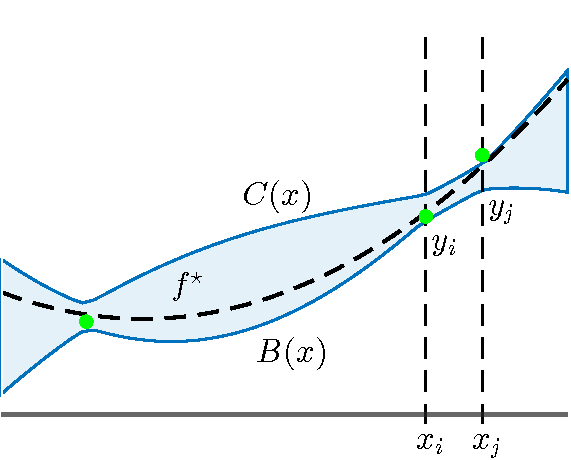
\includegraphics[scale=0.5]{../images/chap2_width_A.pdf} \hspace{8pt}
	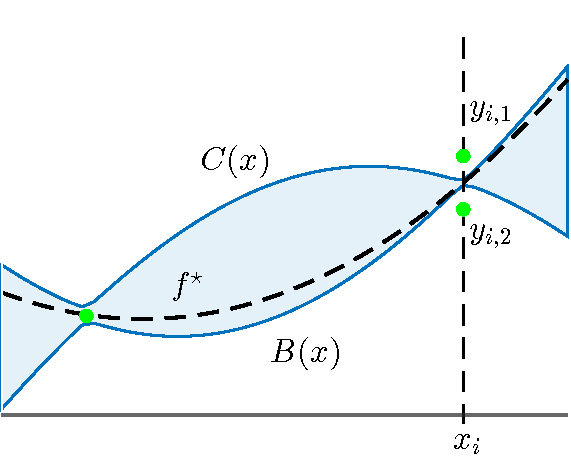
\includegraphics[scale=0.5]{../images/chap2_width_B.pdf}
	\caption{(Left) A sample lying outside of the uncertainty envelope, implying that the width is smaller than $\bar \delta$ at $x_j$. (Right) Redundant information is used to shrink the uncertainty envelope. In this scenario, we recover the ground-truth value at $x_i$ as $\text{C}(x_i) = \text{B}(x_i) = f^\star(x_i)$.}
	\label{fig.riskBound}
\end{figure}

\begin{proposition} 
	\label{prop.smallWidth}
	{\normalfont \textbf{(Width smaller than the noise bound):}}
	If $\exists \mathsf{y}_i$ such that $y_{i,j} > {\normalfont C}(x_i)$ or $y_{i,j} < \text{B}(x_i)$ for some $j$, then $\text{C}(x_i) - \text{B}(x_i) \leq \bar \delta$.
\end{proposition}
\begin{my_proof}
	Follows from $\text{C}(x_i) \geq \text{B}(x_i)$, $\text{C}(x_i) \leq y_{i,j} + \bar \delta$ and $\text{B}(x_i) \geq y_{i,j} - \bar \delta$ for any $i=1,\dots,d$ and any $j=1,\dots,n_i$. 
\end{my_proof} 

Suppose now one has sampled $(x_i,\mathsf{y}_i)$ with $\mathsf{y}_i = \begin{bmatrix} y_{i,1} & y_{i,2} \end{bmatrix}^\top$, $y_{i,1} = f^\star(x_i) + \bar \delta$ and $y_{i,2} = f^\star(x_i) - \bar \delta$. Then there is no uncertainty whatsoever about $f^\star$ at $x_i$ since $f^\star(x_i) = (y_{i,1} + y_{i,2})/2$ is the only possible value attainable by the ground-truth. This illustrates that the possibility of having multiple outputs at the same location allows for the uncertainty interval to shrink past the $\bar \delta$ width, and eventually even reduce to a singleton as shown in Figure~\ref{fig.riskBound} (right). Notwithstanding, the addition of a new datum to an existing dataset|be it in the form of a new output at an already sampled location or a completely new input-output pair|can only reduce the uncertainty.

\begin{proposition} 
	\label{prop.decreasing}
	{\normalfont \textbf{(Decreasing uncertainty)}}
	Let $C_{{\normalfont 1}}(x)$ denote the solution of $\mathds{P}1$ with a dataset $D_1 = \{(x_i,\mathsf{y}_i)\}_{i=1}^{d}$, and $C_{{\normalfont 2}}(x)$ the solution with $D_2 = D_1 \cup \{(x_{d+1},\mathsf{y}_{d+1})\}$. Then $C_{{\normalfont 2}}(x) \leq C_{{\normalfont 1}}(x)$ for any $x \in \Omega$. 
\end{proposition}
\begin{my_proof}
	Given in Section~\ref{sec.selected_derivations}.
\end{my_proof}

%Let us take a closer look at the tightened constraint \eqref{eq.tightenedConstr}. The term $\bar c^\top K_{\bar X \bar X}^{-1} K_{\bar X z} =: s(z)$ represents an interpolating model passing through the output values $\bar c$, that is, $c$ and $c_x$ (see e.g. the discussion in Section~3.1 of \cite{maddalena2020deterministic}). If the difference $s(z) - c_z$ can be made small, then the tightening will also be reduced, whereas it will be significant if the difference is large. The result is of course dictated by the $\infty$-norm constraint, since $c_z$ cannot be more than $\bar \delta$ away from all the outputs $\mathsf{y}$ available at $z$. Therefore, a new datum will cause significant shrinkage of the envelope at a point $z \in \Omega$ when the new output causes $s(z) - c_z$ to be large, which intuitively can be seen as a measure of gained information through the new sample. Finally, this process is weighted by the inverse of the power function $P_{\bar X}^{-2}(z)$, which does not depend on any output, but only on the input locations. This indicates the advantage of evenly-spaced samples over random or bulked ones on the overall bound width. Example~1 in Section~\ref{sec::Result} confirms this intuition.

\begin{remark}
	Recovering the ground-truth as shown in Figure~\ref{fig.riskBound} (right) requires the noise realizations to match $\bar \delta$ and $-\bar \delta$; it is thus necessary to have tight noise bounds for it to happen. On the other hand, Proposition~\ref{prop.decreasing} guarantees the decreasing uncertainty property regardless of how accurate $\bar \delta$ is. Although not explicitly stated, a completely analogous result holds for the lower part of the envelope $\text{B}(x)$.
\end{remark}

\subsection{A sub-optimal solution}

The discussion in this subsection assumes that only one sample is present at each input location, i.e., $\mathsf{y}_i = y_i$ for $i=1,\dots,d $, so that $\mathsf{y}=y$.

In order to alleviate the computational complexity of having to solve two optimization problems at each query point, closed-form expressions can be employed instead. These surrogates yield sub-optimal bounds around any pre-specified kernel model of the form $s(x) = \alpha^\top K_{Xx}$, for some $\alpha \in \mathbb{R}^d$. 
\begin{proposition}
	\label{prop:uniform}
	Let $s(x)=\alpha^\top K_{Xx}$, for a given $\alpha \in \mathbb{R}^d$. Then, for any $x\in \Omega$, the ground-truth is bounded by $s(x) - S(x) \leq f^\star(x) \leq s(x) + S(x)$ with
	\begin{empheq}[box={\mymathbox[colback=black!2,drop small lifted shadow, sharp corners]}]{equation}
	%\begin{equation}
		S(x) =  P_X(x) \, \sqrt{ \Gamma^2 + \tilde\Delta } + \bar{\delta} \, \onenorm{K_{XX}^{-1}K_{Xx}} + \, \vert \tilde{s}(x) - s(x) \vert
		\label{eq.uniformBound2}
	%\end{equation}
	\end{empheq}
	where $\tilde{s}(x) = y^\top K_{XX}^{-1} K_{Xx}$, and the constant $\tilde\Delta$ is the minimum of the unconstrained convex problem $\min_{\nu \in \mathbb{R}^d} \left\{ \frac{1}{4}\nu^\top K_{XX}\nu + \nu^\top y + \bar{\delta} \onenorm{\nu}\right\}$.
\end{proposition}
\begin{proof}
	See Appendix~\ref{app.lemproof}.
\end{proof}

The map $\tilde{s}(x) = y^\top K_{XX}^{-1} K_{Xx}$ is an interpolant for the available outputs $y$. Note also that none of the terms in \eqref{eq.uniformBound2} depend on the model weights $\alpha$ with the exception of the last term $|\tilde s(x) - s(x)|$. Therefore, the width $S(x)$ will be minimized when $s(x) = \tilde s(x) \implies \alpha = y^\top K_{XX}^{-1}$. Since such a model would severely overfit, a balance between smoothing the data and not diverging too much from $\tilde s(x)$ has to be found. In our previous work \cite{maddalena2020deterministic}, we have illustrated how kernel ridge regression and minimum norm models are good candidate techniques to accomplish this goal.

By reformulating the optimal bounds, we uncover their relation with the suboptimal estimates given in Proposition~\ref{prop:uniform}. First, consider $\mathds{P}1$ and optimize over the decision variable $\delta = c - y$ rather than over $c$. Next, apply a quadratic decomposition identical to the one used in \eqref{eq.quadraticDecomp} to the complexity constraint \eqref{eq.P2constrA} and solve for $c_x$. After recalling that $\tilde{s}(x) = y^\top K_{XX}^{-1} K_{Xx}$ and $\rknorm{\tilde s}^2 = y^\top K_{XX}^{-1} y$, one obtains
\begin{equation}
	\begin{aligned}
		c_x  \leq \;&  P(x) \sqrt{ \Gamma^2 - \rknorm{\tilde s}^2 - \delta^\top K_{XX}^{-1}\delta +2y^\top K_{XX}^{-1}\delta} +\tilde s(x) 
		+ \delta^\top K_{XX}^{-1}K_{Xx}
	\end{aligned}	
	\label{eq.ineq}
\end{equation}
Instead of maximizing $c_x$, the right-hand side of \eqref{eq.ineq} can be directly considered as the objective function equivalently. As a result, we obtain 
\[
\begin{aligned}
	\max_{\infnorm{\delta} \leq \bar \delta}\;\;& \tilde s(x) + P(x) \sqrt{ \Gamma^2 - \rknorm{\tilde s} - \delta^\top K_{XX}^{-1}\delta -2y^\top K_{XX}^{-1}\delta} + \delta^\top K_{XX}^{-1}K_{Xx} 
\end{aligned}
\]
Now, relax the problem by allowing $\delta$ to attain different values inside and outside the square-root
\begin{subequations}
	\begin{align}\notag
		\max_{\delta_1,\delta_2 \in \mathds{R}^{d}} &  \tilde s(x) + P(x) \sqrt{ \Gamma^2 - \rknorm{\tilde s}^2 - \delta_1^\top K_{XX}^{-1}\delta_1 +2y^\top K_{XX}^{-1}\delta_1} + \delta_2^\top K_{XX}^{-1}K_{Xx} \\ \label{eq.relaxedObjective}
		\text{\normalfont subj. to} & \;\; \; \infnorm{\delta_1} \leq \bar \delta, \; \infnorm{\delta_2} \leq \bar \delta 
	\end{align}
\end{subequations}
Note that the objective is separable and that $\tilde\Delta$ is the dual solution of 
\begin{equation}
	\max_{\delta_1 \in \mathbb{R}^d} \left\{ -\delta_1^\top K_{XX}^{-1}\delta_1 + 2y^\top K_{XX}^{-1}\delta_1 - \rknorm{\tilde s}^2 \right\}
\end{equation}
Also, $\max_{\delta_2 \in \mathbb{R}^d} \{ \delta_2^\top K_{XX}^{-1}K_{Xx} : \infnorm{\delta_2} \leq \bar\delta \} = \bar{\delta} \onenorm{K_{XX}^{-1}K_{Xx}}$ since these norms are duals of each other. Remember that the objective \eqref{eq.relaxedObjective} is a conservative upper bound for $f^\star(x)$, having $\tilde s(x)$ as the reference model. Given any smoother $s(x)$, the triangle inequality $|f(x) - s(x)| \leq |f(x) - \tilde s(x)| + |\tilde s(x) - s(x)|$ can be used to bound the distance between its predictions and the ground-truth values, arriving thus at the same expressions presented in Proposition~\ref{prop:uniform}.

From \eqref{eq.ineq}, the noise variable $\delta$ is seen to increase the maximum in two distinct ways: through the inner product $\delta^\top K_{XX}^{-1}K_{Xx}$, and via a norm augmentation corresponding to $\tilde\Delta$. One source of conservativeness in Proposition~\ref{prop:uniform} is taking into account the worst-possible inner-product and norm increase jointly. Despite this fact, they yield competitive results for moderate noise-levels as shown numerically in Section~\ref{sec::Result}. We moreover note that in the noise-free scenario, \eqref{eq.ineq} and \eqref{eq.relaxedObjective} are the same, and Proposition~\ref{prop:uniform} simplifies to the classical bounds in the interpolation case (see for instance \cite{fasshauer2011positive}).

\begin{remark}
	The sub-optimal bounds presented in this subsection feature a nominal model at their center, which is desirable in many practical situations. In the optimal scenario, the minimum norm regressor $s^\star(x) = \alpha^{\star\top} K_{Xx}$, $\alpha^\star = \text{arg}\min_{\alpha \in \mathbb{R}^d} \{ \alpha^\top K_{XX} \alpha : \infnorm{K_{XX} \alpha - y} \leq \bar\delta \}$ can be used as a nominal model. This choice is guaranteed to lie completely within $\text{C}(x)$ and $\text{B}(x)$|although not necessarily in the middle|since the map $s^\star$ belongs to $\mathcal{H}$ and is a feasible solution for $\mathds{P}0$.
\end{remark}

\section{Numerical examples}

\section{Selected derivations}
\label{sec.selected_derivations}

Proof of Proposition~\ref{prop.decreasing}.

\begin{my_proof}
		Denote by $\mathds{P}1_1$ the problem solved with $D_1$ and decision variables $\begin{bmatrix} c & c_x \end{bmatrix}$. Similarly, $\mathds{P}1_2$ is associated with the dataset $D_2$ and the decision variables $\begin{bmatrix} c & c_x & c_z \end{bmatrix}$, where $c_z$ are due to the additional input in $D_2$. Since $D_2$ contains all members of $D_1$, the $\infty$-norm constraint of $\mathds{P}1_2$ can be recast as that of $\mathds{P}1_1$ and an additional constraint for $c_z$ and the new outputs. Let $\mathds{X}  := X \cup \{x\}$, $\bar c := \begin{bmatrix} c^\top c_x \end{bmatrix}^\top$ and $z := x_{d+1}$ be shorthand variables to ease notation. The complexity constraint of $\mathds{P}1_2$ is then
		\begin{subequations}
			\begin{align}
				\begin{bmatrix}
					\bar c \\
					c_z
				\end{bmatrix}^\top 
				\begin{bmatrix}
					K_{\mathds{X} \mathds{X} } & K_{\mathds{X}  z} \\
					K_{z \mathds{X} } & k(z,z)
				\end{bmatrix}^{-1} 
				\begin{bmatrix}
					\bar c \\
					c_z
				\end{bmatrix} & \leq \Gamma^2 \\
				%
				\overset{(i)}{\Leftrightarrow}
				\bar c^\top K_{\mathds{X} \mathds{X} }^{-1} \bar c +
				P_{\mathds{X} }^{-2}(z) \, 
				%\begin{bmatrix}
				%	\bar c \\
				%	c_z
				%\end{bmatrix}^\top
				%\begin{bmatrix}
				%	K_{\bar X \bar X}^{-1} K_{\bar X z} \\
				%	-1
				%\end{bmatrix}
				\left\|
				\begin{bmatrix}
					K_{\mathds{X} \mathds{X} }^{-1} K_{\mathds{X} z} \\
					-1
				\end{bmatrix}
				\begin{bmatrix}
					\bar c \\
					c_z
				\end{bmatrix}\right\|_2^2
				& \leq \Gamma^2 \\
				%
				\overset{(ii)}{\Leftrightarrow} \;
				\begin{bmatrix}
					c \\
					c_x
				\end{bmatrix}^\top 
				\begin{bmatrix}
					K_{XX} & K_{Xx} \\
					K_{xX} & k(x,x)
				\end{bmatrix}^{-1} 
				\begin{bmatrix}
					c \\
					c_x
				\end{bmatrix} \label{eq.tightenedConstr}%\\\notag
				+
				P_{\mathds{X} }^{-2}(z) \, \left( \bar c^\top K_{\mathds{X} \mathds{X} }^{-1} K_{\mathds{X} z} - c_z \right)^2 
				&\leq \Gamma^2 
			\end{align}
			\label{eq.quadraticDecomp}
		\end{subequations}
		where the matrix identity found in Appendix~\ref{app.blockMatrixIdent} was used in $(i)$ and $P^2_{\mathds{X} }(z) = k(z,z) - K_{z \mathds{X} } K_{\mathds{X} \mathds{X} }^{-1} K_{\mathds{X} z}$. In $(ii)$, the definitions of $\bar c$ and $\mathds{X} $ were used. Thanks to $P_{\mathds{X} }(z) \geq 0, \forall z$ and the quadratic term multiplying it, we conclude that for any choice of the decision variable $c_z$, \eqref{eq.tightenedConstr} is a tightened version of the complexity constraint of $\mathds{P}1_1$, which is \eqref{eq.P2constrA}. As a result, the maximum of $\mathds{P}1_2$ is lower or equal than that of $\mathds{P}1_1$. 
\end{my_proof}